\documentclass[11pt]{article}
\usepackage[margin=1in]{geometry}
\usepackage{graphicx}
\graphicspath{{images/}}
\usepackage{float}
\usepackage[T1]{fontenc}

\begin{document}
\title{\huge Projet d'algorithmique et bioinformatique}
\author{Groupe 6 :\\
HUYLENBROECK Florent\\
TCHANME Paul}
\date{18 Décembre 2020}
\maketitle
\newpage
\section{Introduction}
Dans le cadre de ce projet, il nous a été demandé, par groupe de deux étudiants, de concevoir un programme d'assemblage de fragments à partir d'une collection de fragments.
Pour cela, nous devions utiliser l'approximation de type \emph{Greedy} (glouton) et l'alignement semi-global. Il nous était aussi imposé de considérer, en plus des fragments, leurs compléments inverses.
\section{Répartition des tâches au sein du groupe}
Lors de la réception des consignes, nous avons d'abord discuté en visioconférence de la manière dont nous allions procéder. Nous avons décidé de répartir les tâches de la manière suivante :\\[.5cm]
Tchanme Paul :
\begin{itemize}
	\item Premier jet des fonctions d'entrées/sorties.
	\item Premier jet des fonctions jusqu'au calcul du chemin hamiltonien.
	\item Ecriture du rapport.
\end{itemize}
Huylenbroeck Florent :
\begin{itemize}
	\item Premier jet du reste des fonctions.
	\item Finalisation des fonctions.
	\item Unification du code (syntaxe).
	\item Correction des bugs.
	\item Ecriture du rapport.
\end{itemize}
Cette répartition a été respectée malgré les difficultés actuelles à travailler en groupe.
\newpage
\section{Démarche}
Les différentes étapes du programme sont les suivantes :
\begin{itemize}
	\item Récupérer l'ensemble de fragments décrit dans un fichier \emph{.fasta} (extension de fichier utilisée pour décrire des séquences de nulcéotides ou d'acides aminés).
	\item Construire l'\emph{overlap multigraph} (le graphe des chevauchements) en considérant les fragments et leurs compléments inverses.
	\item Dans ce graphe, rechercher un chemin hamiltonien avec l'approximation de type Greedy.
	\item Sur base de ce chemin, construire la séquence consensus.
	\item Ecrire cette séquence et son complément inverse dans deux fichiers fasta de sortie.
\end{itemize}
\subsection*{Approche}
Le point qui nous a demandé réflexion a été la gestion des compléments inverses. En effet lors de la recherche d'un chemin hamiltionien dans le graphe des chevauchements, nous ne pouvions considérer qu'une seule version de chaque fragment. Cependant il fallait que chaque version de chaque fragment soit présente au début du calcul.\\
Notre solution fut de considérer, pour chaque paire de fragments, 4 liens. Soit fragment1, fragment2 deux fragments, les liens considérés dans le graphe de chevauchement sont :
\begin{itemize}
	\item (fragment1)$\rightarrow$(fragment2)
	\item (fragment1)$\rightarrow$(fragment2\_ic)
	\item (fragment1\_ic)$\rightarrow$(fragment2)
	\item (fragment1\_ic)$\rightarrow$(fragment2\_ic)
\end{itemize}
Où fragmentX\_ic est le complément inverse du fragment X.
Il existe 4 autres liens envisageable, mais il sont équivalents un à un aux liens ci-dessus. Par exemple, le lien (fragment2)$\rightarrow$(fragment1) est équivalent à (fragment1\_ic)$\rightarrow$(fragment2\_ic).
\subsection*{Optimisations}
\subsubsection*{Types et structures de données utilisée}
Pour stocker les fragments, nous avons choisi d'utiliser des tableaux de \emph{byte}. En effet, chaque nucléotide d'un fragment ne demande que 3 bits pour conserver toute l'information (5 états différents ${a,c,g,t,-}$). Le type de donnée de plus faible taille, pouvant contenir cette information est le byte car celui ci occupe 8 bits ce qui permet de stocker 255 valeurs différentes.\\
De manière générale les tableaux ont été favorisés au maximum.\\[.5cm]
En ce qui concerne le graphe des chevauchements, plutot que de construire un graphe dans une structure de données "élaborée" nous avons décidé de ne considérer que la matrice d'adjacence de celui-ci, étant donné que les noeuds (\emph{i.e.} les fragments) sont déjà stockés dans notre programme.\\
Ainsi, le graphe est décrit par un tableau à 3 dimensions d'entiers (le choix d'un type de donnée plus restreint n'était pas envisageable, étant donné que nous ne connaissons pas à l'avance les valeurs maximales atteignables par les scores d'alignements). Les premières et deuxième dimensions sont de la taille de l'ensemble des fragments. La troisième dimension est de taille 4, elle contient les 4 scores d'alignements décrits dans la sous-section \emph{Approche}.\\[.5cm]
\subsubsection*{Algorithmes}
Directement après la récupération des fragments, ceux ci sont soumis à une étape de tri supprimant tout fragment complètement contenu dans un autre, ou dans le complément inverse d'un autre.\\[.5cm]
L'algorithme de construction de la matrice de chevauchement a été amélioré afin de ne garder en mémoire, à tout moment, qu'un vecteur $a$. En effet, la valeur de chaque entrée de cette matrice ne dépend que de 3 valeurs voisines à cette entrée. De plus seule la toute dernière valeur (au sens des indices) de cette matrice est intéressante. Il n'est donc pas nécessaire de garder en mémoire la matrice complète.\\
Une autre fonction, gardant en mémoire toute la matrice et la retournant a cependant été implémentée afin de procéder à la reconstruction du contig.\\
\subsection*{Changements apportés}
Lors de la recherche d'un chemin hamiltonien, l'approximation Greedy décrite dans le cours à du être adaptée à notre matrice d'adjacence. Ainsi, lorsqu'un arc de poids maximal est séléctionné, une étape de vérification a lieu afin de vérifier que le complément inverse d'au moins un des deux noeuds n'a pas déjà été selectionné. Si c'est le cas l'arc n'est pas selectionné.\\
Pour garder une trace des noeuds considérés, les vecteurs $in$ et $out$ ont été adaptés. Si le complément inverse d'un fragment est séléctionne, la valeur insérée dans ces vecteurs sera $-1$.\\
De plus, la même idée est utilisée pour le vecteur décrivant le chemin hamiltonien. Si le noeud traversé est un complément inverse, alors sa valeur dans le chemin sera négative. Exemple d'un vecteur décrivant un chemin hamiltonien :
$$[1, -2, 7, 6, 4, -5, 3, 0]$$
On remarque que le troisième et sixième fragments sont compléments inverse de leur fragments originaux.\\[.5cm]
Nous avons aussi appliqué les modifications lors de la construction de la matrice de chevauchement permettant de favoriser les gaps en début et fin de séquence comme décrite dans le cours.
\subsection*{Points forts}
Au vu des points évoqués ci-dessus, nous pensons que notre programme est assez rapide pour les étapes jusqu'à la construction de la séquence consensus.
\subsection*{Points faibles, erreurs}
La construction de la séquence consensus donne une séquence en "morceaux" par rapport à la séquence cible. (voir \emph{Résultats}). 
\section{Résultats}
\subsection*{Collection 1}
\begin{figure}[H]
\centering
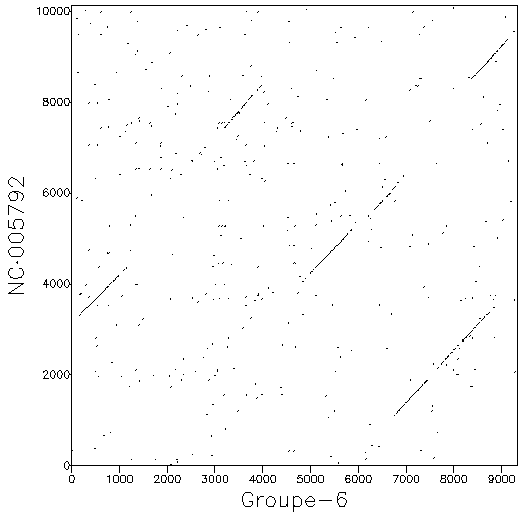
\includegraphics[scale=.55]{10000.png}
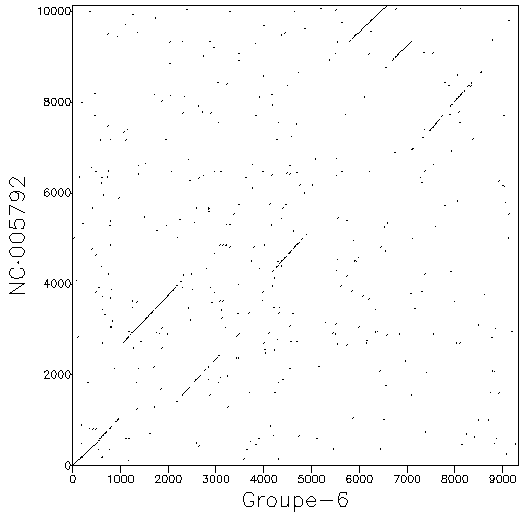
\includegraphics[scale=.55]{10000ic.png}
\caption{dotmatcher des séquences obtenues pour la collection 1 (complément inverse à droite)}
\end{figure}
\subsection*{Collection 2}
Cette collection s'est averée trop volumineuse pour être calculée en un temps raisonnable par notre programme. Nous n'avons donc pas obtenu de résultats pour celle-ci.
\subsection*{Collection 4}
\begin{figure}[H]
\centering
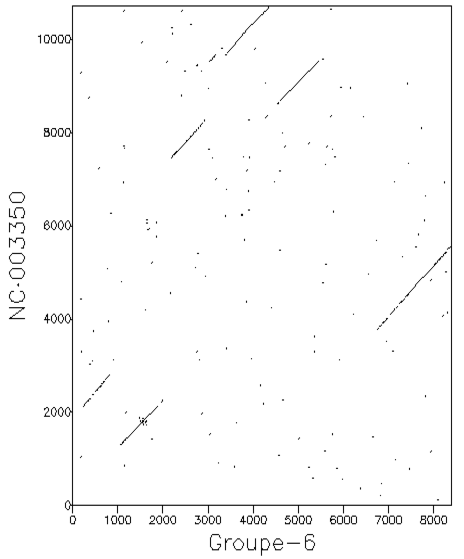
\includegraphics[scale=.55]{11200.png}
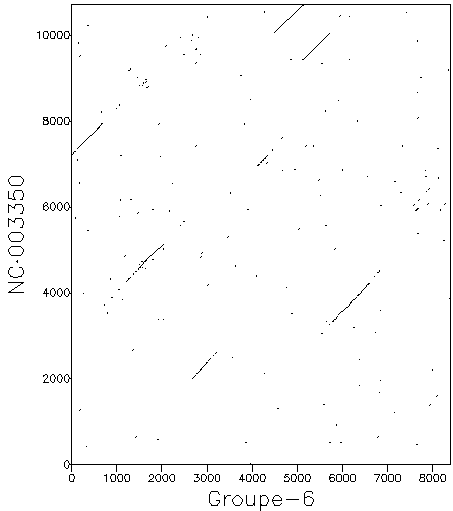
\includegraphics[scale=.55]{11200ic.png}
\caption{dotmatcher des séquences obtenues pour la collection 4 (complément inverse à droite)}
\end{figure}
\subsection*{Collection 5}
\begin{figure}[H]
\centering
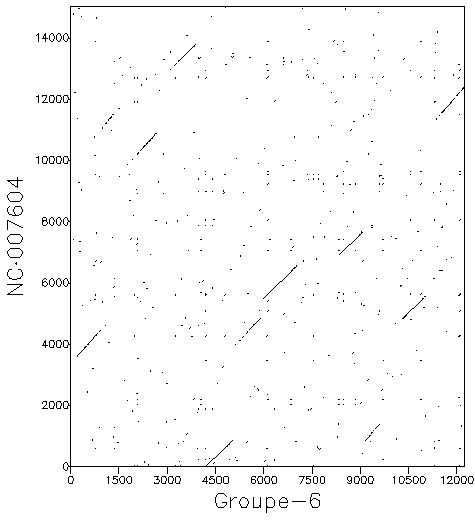
\includegraphics[scale=.55]{16320.png}
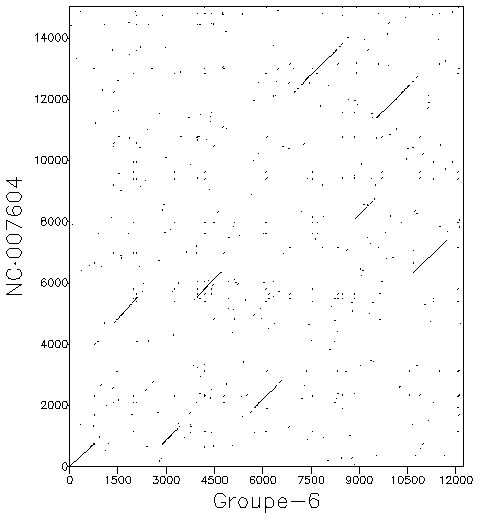
\includegraphics[scale=.55]{16320ic.png}
\caption{dotmatcher des séquences obtenues pour la collection 5 (complément inverse à droite)}
\end{figure}
\newpage
\subsection*{Commentaires et interprétation}
Notre commentaire au sujet des résultats sera global, étant donné la similitude des résultats obtenus.\\
Les séquences construites semblent couvrir en majorité la séquence cible. Cependant nous n'obtenons pas une diagonale parfaite mais plusieurs morceaux de diagonale. Cela est du à une erreur de consensus ou au parcours hamiltionien considéré pour construire ces séquences.
\section{Utilisation de FragmentAssembler}
Pour utiliser \emph{FragmentAssembler.jar}, la ligne de commande doit être formatée comme suit :
\begin{center}
java -jar FragmentAssembler.jar <fichier.fasta> -out <fichier-out.fasta> -out-ic <fichier-out-ic.fasta>
\end{center}
Avec \emph{fichier.fasta} le fichier d'entrée contenant la collection de fragments, \emph{fichier-out.fasta} le fichier de sortie pour la séquence consensus et \emph{fichier-out-ic.fasta} le fichier de sortie pour le complément inverse de la séquence consensus.\\
Les collections fournies avec le projet sont disponibles sous \emph{ressources/Collections/}.
\section{Conclusion}
Nous avons trouvé ce projet intéressant car c'est une application assez concrète de ce qui a été vu en cours, contrairement a certains projets trop abstraits.\\
Nous avons rencontrés certaines difficultés pour communiquer efficacement au sujet de ce projet, malgré l'utilisation de \emph{Github} et d'outils de communication en ligne. Mais cela est du à la période spéciale que nous traversons et au final cela ne nous aura pas porté préjudice.\\
La difficulté majeure du projet pour nous a été le calcul de la séquence consensus. Nous avons pris notre temps de générer des exemples et de les calculer à la main, afin d'envisager les cas spéciaux d'alignement.\\
Au final nous sommes satisfait des séquences que nous obtenons, malgré qu'elle ne soient pas parfaites.\\
\end{document}